\begin{savequote}[8cm]
Simplicity is prerequisite for reliability.
  \qauthor{--- Edsger W. Dijkstra}
\end{savequote}

\chapter{An introduction to high-level modular assembly}

\minitoc

Already from the start, the field of structural DNA nanotechnology has been interested in modular assemblies, although then mostly in the form of infinite chrystal structures. Allegedly, Ned Seeman was inspired to pioneer the field after seeing the artwork \emph{Depth} by M.C. Escher.

This chapter will provide an overview on the background of self-assembled multi-component structures, starting with experimental results of ever-increasing size and followed by a selection of theoretical models.

\section{Experimental applications} \label{sec:experimental_appl}
From small tiles made from a handful of strands to megadalton-scale structures made from multiple origamis, modular assembly has seen a lot of experimental research. This section will detail some results of particular interest to the polycube model presented in Chapter \ref{ch:3-polycubes}.

\subsection{DNA tiles and bricks}
% Tiles: https://www.nature.com/articles/28998

\begin{figure}[h]
  \centering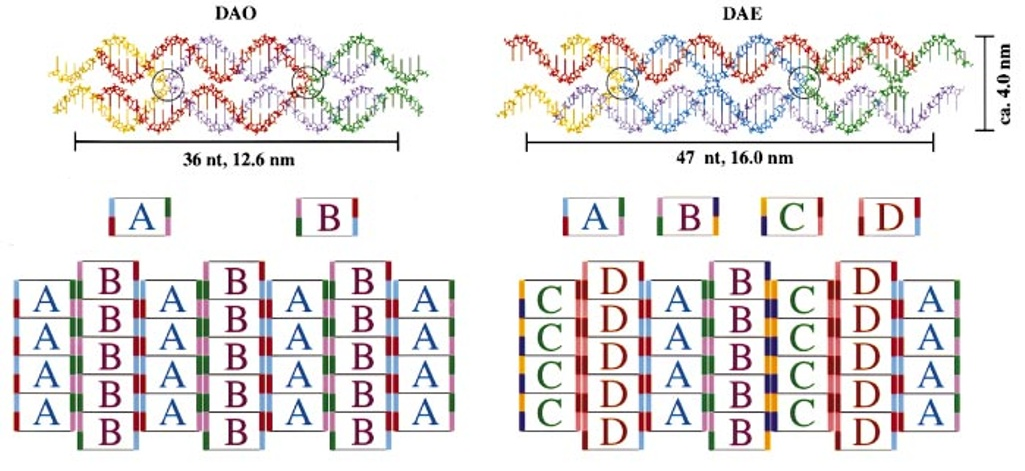
\includegraphics[width=\textwidth]{figures/dna_tiles.png}
  \caption{DX tiles forming 2D lattices, adapted from \cite{winfree1998design}. a) Lattices made from two units and four units respectively. b) Examples of DAO and DAE tile designs.}
  \label{fig:dna_tiles}
\end{figure}

% Bricks: https://www.nature.com/articles/nature24648

\begin{figure}[h]
  \centering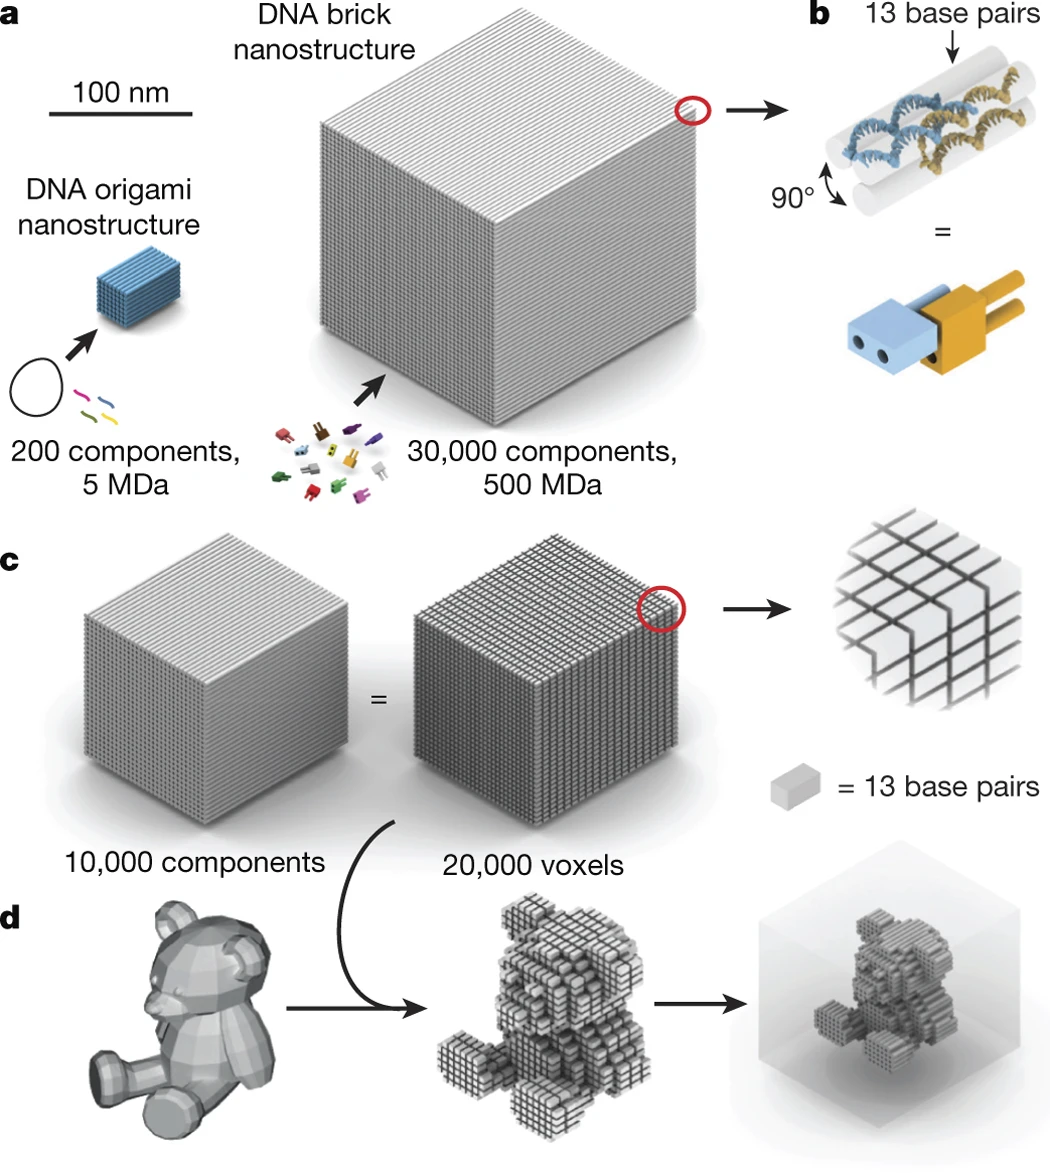
\includegraphics[width=0.6\textwidth]{figures/dna_bricks.png}
  \caption{3D bricks from \cite{ong2017programmable}}
  \label{fig:dna_tiles}
\end{figure}

\subsection{RNA tiles}
%https://www.science.org/doi/abs/10.1126/science.1253920 
In 2014, Cody Geary published a method of folding RNA tiles co-transcriptionally \cite{geary2014single}. The design used a set of tertiary RNA motifs, such as kissing hairpins and double crossovers, to fold the RNA strand into the desired tile structure. The tiles then assembled connected by complementary 120-degree kissing loop interactions. The design method was later described in depth in the \emph{Methods in Molecular Biology} book series \cite{sparvath2017computer}.

\begin{figure}[h]
  \centering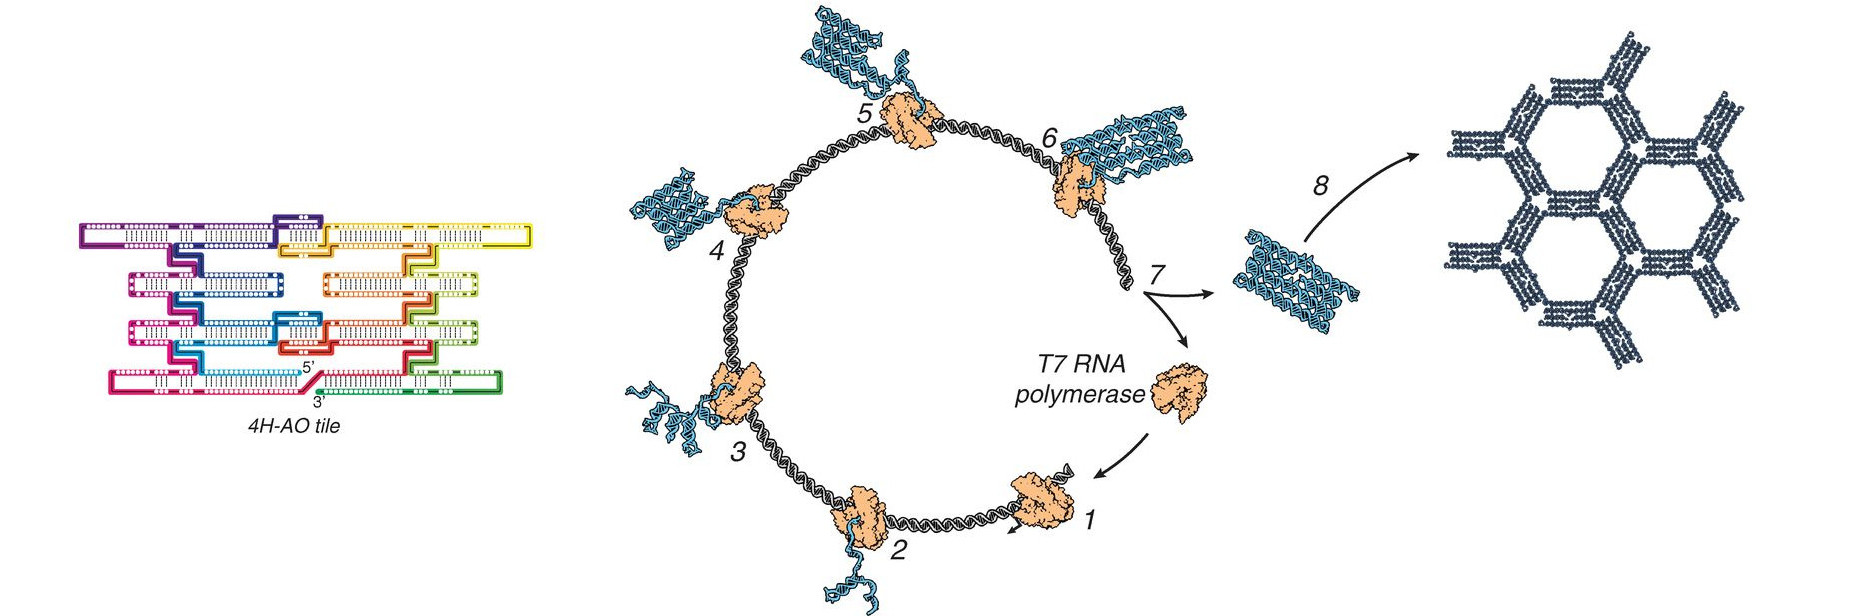
\includegraphics[width=\textwidth]{figures/rna_tiles.jpeg}
  \caption{2D RNA tiles from \cite{geary2014single}}
  \label{fig:rna_tiles}
\end{figure}

\subsection{DNA origami arrays}\label{sec:origamiArrays}
% https://www.nature.com/articles/nature24655

In 2017, Tikhomirov, et al.\cite{tikhomirov2017fractal} demonstrated two-dimensional patterns assembled on the micrometre-scale using square origami tiles connecting through their complementary edges. helices

\begin{figure}[h]
  \centering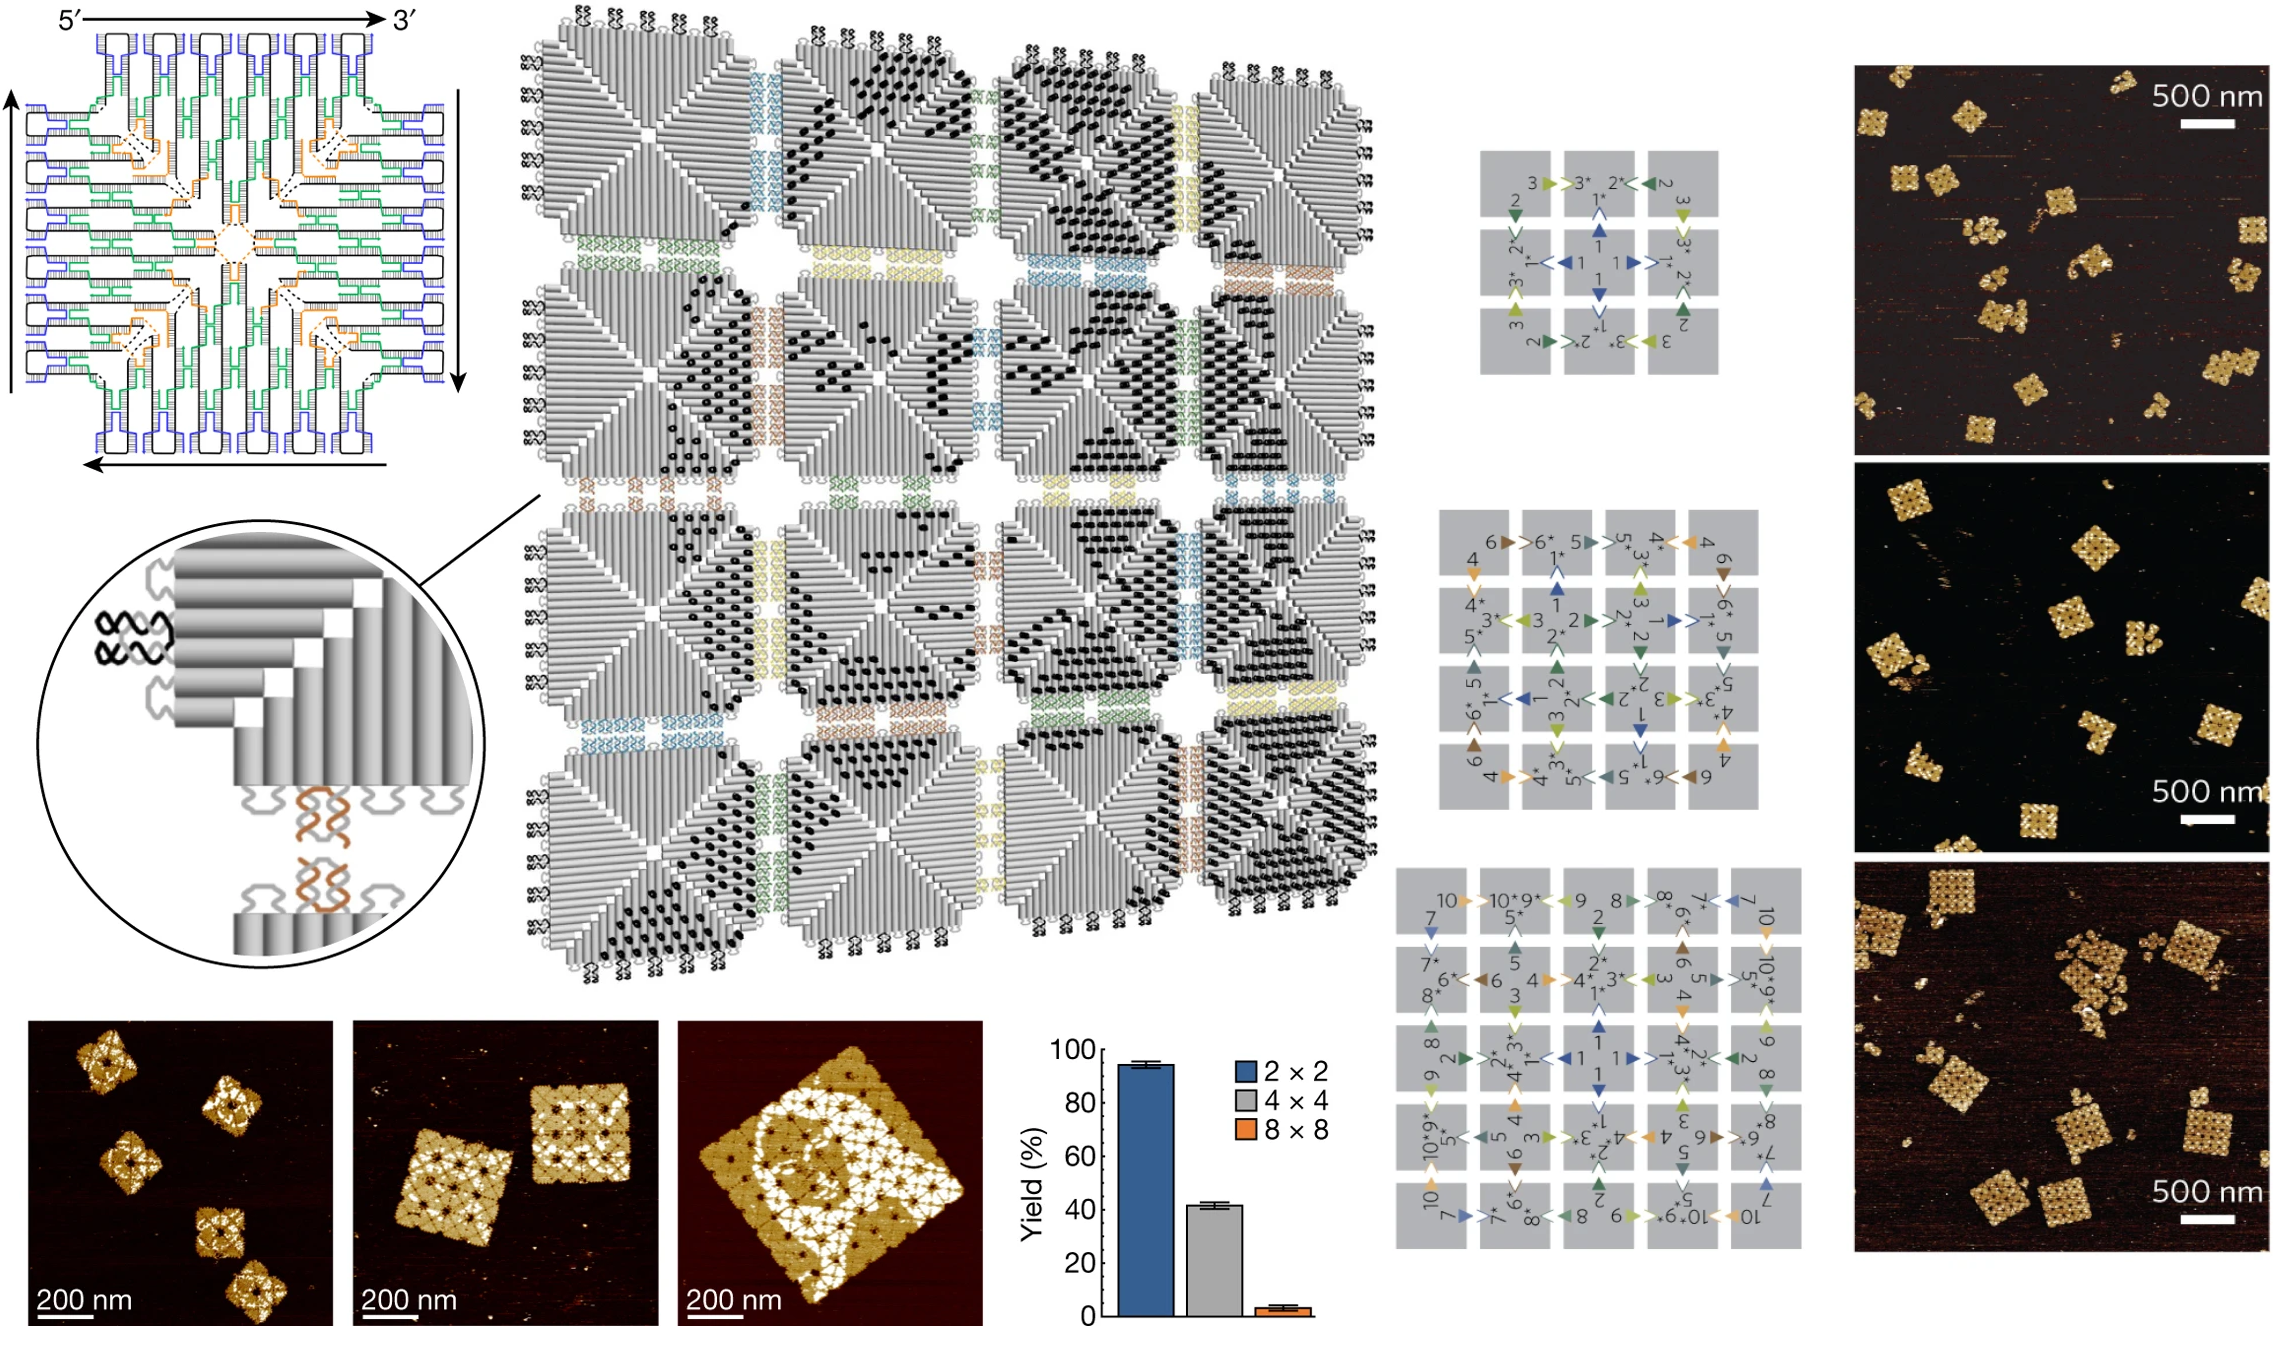
\includegraphics[width=0.6\textwidth]{figures/monalisa_tiles.png}
  \caption{Adapted from \cite{tikhomirov2017fractal}}
\end{figure}

\subsection{Shape-complementary origami}
% 2D https://www.nature.com/articles/nchem.1070
% 3D https://science.sciencemag.org/content/347/6229/1446.abstract

Also in 2017, Wagenbauer, et al. \cite{wagenbauer2017gigadalton} used shape-complementarity to assemble origami tiles into three-dimensional polyhedral shapes up to 450 nanometers in diameter.


\subsection{DNA origami nanochambers}
% https://pubs.acs.org/doi/full/10.1021/jacs.0c07263

\begin{figure}[h]
  \centering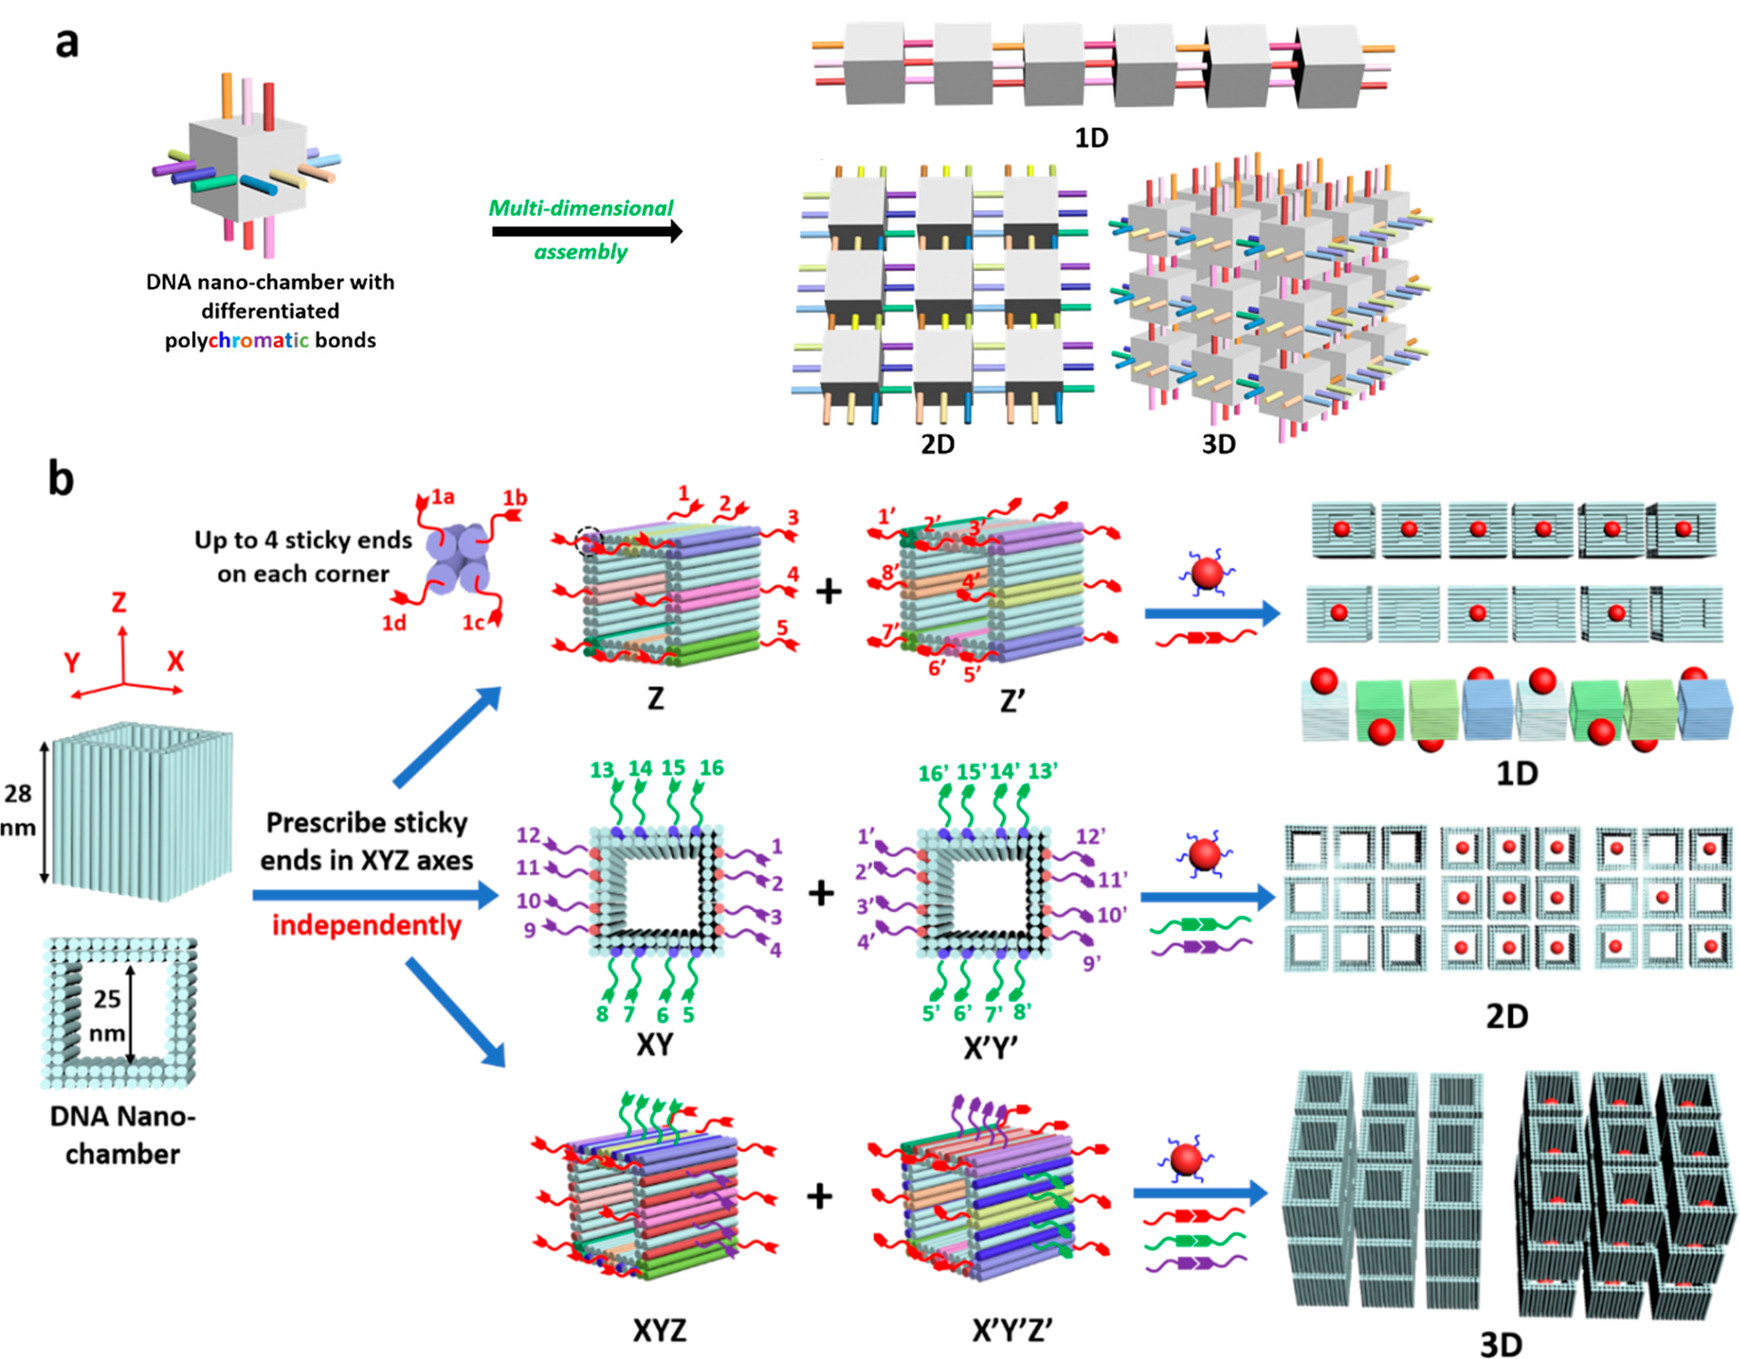
\includegraphics[width=\textwidth]{figures/nanochambers2.jpeg}
  \caption{DNA nanochambers, adapted from}
\end{figure}

\subsection{Octahedral DNA origami frames}
% https://onlinelibrary.wiley.com/doi/abs/10.1002/anie.201913958

\begin{figure}[h]
  \centering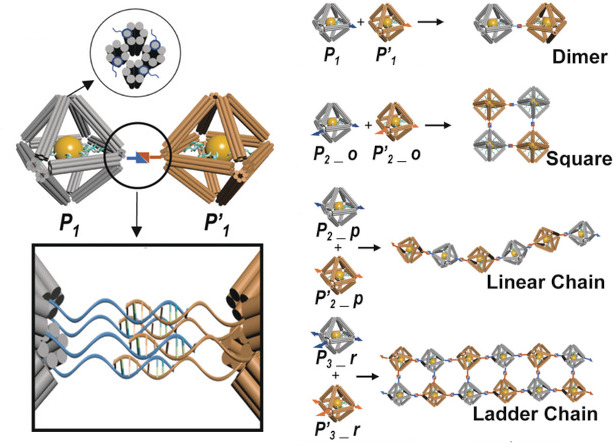
\includegraphics[width=\textwidth]{figures/tian.jpg}
  \caption{Octahedral DNA origami frames, adapted from}
\end{figure}


\section{Tile assembly models}
It would be computationally unreasonable to simulate module assemblhelicesy at the level of individual nucleotides. A better approach is instead to use an abstract model to predict the assembly process with the modules treated as rigid bodies. This section will present earlier such models as a background to my own model described in Chapter \ref{ch:3-polycubes}.

\subsection{Wang tiles}
Introduced by Hao Wang in 1961 \cite{wang1961proving}, so called \emph{Wang tiles} are 

\begin{figure}[h]
  \centering\includesvg[width=0.6\textwidth]{figures/Wang_11_tiles.svg}
  \caption{Wang tiles}
\end{figure}

\subsection{The algorithmic tile assembly model}

% David Doty overview: https://cacm.acm.org/magazines/2012/12/157881-theory-of-algorithmic-self-assembly/fulltext

In his 1998 thesis Erik Winfree showed the usage of the double-crossover (DX) motif to create regular arrays \cite{winfree1998design}. These tiles behave like Wang tiles\cite{wang1961proving} and do not allow rotations or reflections. Winfree also investigated the possibility of using such tiles for computation \cite{winfree1998algorithmic}.
% DX array https://www.nature.com/articles/28998

Co-operative binding

\begin{figure}[h]
  \centering\includesvg[width=\textwidth]{figures/atam.svg}
  \caption{Algorithmic self-assembly model}
\end{figure}

\subsection{The polyomino model}\label{sec:polyomino}

The main inspiration for the polycube model presented in Chapter \ref{ch:3-polycubes} is the polyomino model \cite{ahnert2010self}\cite{johnston2011evolutionary}. The main difference to aTAM is that polyomino tiles are allowed to rotate. They also have a constant binding strength (in other words, it is a temperature-1 model).

%, studying the self-assembly, modularity and evolutionary dynamics of \emph{polyominoes}.

Polyominoes are abstract structures composed of one or more squares, connected by their edges. The polyomino assembly model developed is similar in assembly to the later experimental micro-meter scale tile designs by Tikhomirov \cite{tikhomirov2017fractal} described in Section \ref{sec:origamiArrays}. Compared to Wang tiles\cite{wang1961proving}, the edge binding does not need to be between edges of the same colour, but can be specified by a more complex interaction matrix. Furthermore, the tiles can be rotated to bind, creating further possibilities for symmetries.

\begin{figure}[h]
    \centering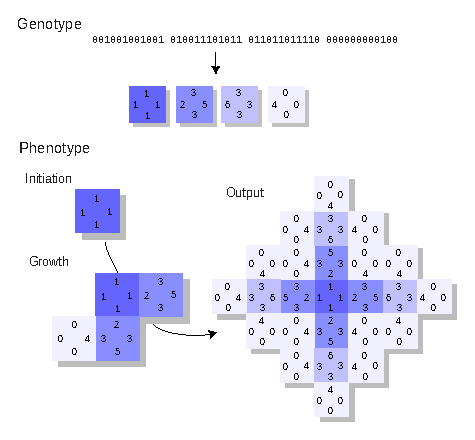
\includegraphics[width=0.6\textwidth]{figures/polyominoes.eps}
    \caption{Illustration of the polyomino assembly model used by Johnston. A \emph{genotype}, in the form of a ruleset of possible tiles, encodes for a polyomino \emph{phenotype}, grown stochastically from an initial seed tile. Image adapted from \cite{johnston2011evolutionary}.}
    \label{fig:polyominoes}
\end{figure}

I aim to build on Johnston's work on polyominoes to explore the properties of such self-assembling systems in three dimensions; the self-assembly of \emph{polycubes}. With such a model in place, it should be possible to design, through shape complementary in DNA origami \cite{wagenbauer2017gigadalton}, kissing interactions in RNA origami \cite{geary2014single}, or other methods, robotic modules with the interfaces necessary to assemble into the desired polycube shape. My current progress within this project is covered in Chapter \ref{ch:3-polycubes}.

\section{Algorithmic Information Theory and input-output maps}

\section{Patchy particle simulation}
